% Rewritten presentation (spacious, rubric-aligned a–e)
% Build: pdflatex Final_Presentation_REWRITE.tex (run twice for TOC)
\documentclass[aspectratio=169, 11pt]{beamer}

\usetheme{Madrid}
\usecolortheme{seahorse}
\setbeamertemplate{navigation symbols}{}
\setbeamertemplate{footline}[frame number]

\usepackage{amsmath, amssymb}
\usepackage{booktabs}
\usepackage{graphicx}
\usepackage{xcolor}
\usepackage{tikz}
\usetikzlibrary{positioning, arrows.meta}

\definecolor{vflblue}{RGB}{41, 128, 185}
\definecolor{vflgreen}{RGB}{39, 174, 96}
\definecolor{vflred}{RGB}{231, 76, 60}
\definecolor{lightbg}{RGB}{248, 249, 250}

\setbeamercolor{frametitle}{bg=vflblue, fg=white}
\setbeamercolor{title}{fg=vflblue}
\setbeamercolor{block title}{bg=vflblue, fg=white}
\setbeamercolor{block body}{bg=lightbg}
\setbeamercolor{block title alerted}{bg=vflred, fg=white}
\setbeamercolor{block title example}{bg=vflgreen, fg=white}

% Figures produced by notebooks already live here
\graphicspath{{./presentation_figures/}{./Part4_figures/}{./presentation_figures_vfu_verification/}{./}}

% Include a figure if it exists; otherwise compile with a placeholder box.
\newcommand{\SlideFig}[2]{%
  \IfFileExists{#1}{%
    \includegraphics[width=#2,height=0.72\textheight,keepaspectratio]{#1}%
  }{%
    \IfFileExists{presentation_figures/#1}{%
      \includegraphics[width=#2,height=0.72\textheight,keepaspectratio]{presentation_figures/#1}%
    }{%
      \IfFileExists{Part4_figures/#1}{%
        \includegraphics[width=#2,height=0.72\textheight,keepaspectratio]{Part4_figures/#1}%
      }{%
        \begin{center}
        \fbox{\parbox{0.86\linewidth}{\centering\vspace{0.9em}\small
        \textbf{Missing figure:} \texttt{#1}\\[0.35em]
        Expected in \texttt{presentation\_figures/} or \texttt{Part4\_figures/}.\\
        Re-run the notebook cells that generate the plots.\vspace{0.9em}}}
        \end{center}%
      }%
    }%
  }%
}

\title[E-VFU]{E-VFU: Multi-Attack Verification for Vertical Federated Unlearning}
\subtitle{Clear rubric-aligned explanation (a–e)}
\author{Gourab Biswas \and Fairuz}
\institute{Undergraduate ML project}
\date{\today}

\begin{document}

\begin{frame}
  \titlepage
\end{frame}

\begin{frame}{Outline (rubric order)}
  \tableofcontents
\end{frame}

% =============================================================================
\section{(a) Problem definition}
% =============================================================================

\begin{frame}{What problem are we solving?}
  \begin{block}{Vertical Federated Learning (VFL)}
    Multiple parties share the \textbf{same users} (aligned IDs) but each holds \textbf{different feature columns}.
    One party typically holds the label $y$.
  \end{block}
  \vspace{0.6em}
  \begin{alertblock}{Unlearning requirement}
    When a party/feature/samples must be removed (e.g., GDPR erasure), the deployed model should behave like it
    \textbf{never learned from the forget target}, without expensive full retraining each time.
  \end{alertblock}
\end{frame}

\begin{frame}{Why ``verification'' matters (not just accuracy)}
  \begin{block}{Two different questions}
    \begin{itemize}
      \item \textbf{Utility}: is the model still good at prediction on test data?
      \item \textbf{Forgetting}: can an attacker still detect whether the model saw the forget target?
    \end{itemize}
  \end{block}
  \vspace{0.6em}
  \begin{alertblock}{Key risk}
    A model can keep high accuracy \emph{and still} leak membership information.
    So we evaluate unlearning with \textbf{multiple verification attacks}, not utility alone.
  \end{alertblock}
\end{frame}

\begin{frame}{Threat model (what an auditor/attacker can do)}
  \begin{block}{What we test}
    \begin{itemize}
      \item \textbf{Output-based MIA (black-box)}: membership inference using only \textbf{model outputs}
            (predicted probabilities \(\hat{y}\) / confidence scores, or logits; optionally derived loss).
      \item \textbf{Gradient-based MIA (stronger access)}: membership inference using \textbf{gradients or gradient statistics}
            (only applicable if such signals are observable in the system).
      \item \textbf{FUMA (forensic)}: detector that uses \textbf{before-vs-after} model behavior on points to spot unlearning artifacts.
      \item \textbf{Shadow-model attack}: train a meta-classifier that asks: does this model look like ``trained on full data'' vs ``retain-only''?
    \end{itemize}
  \end{block}
  \vspace{0.4em}
  \small Passing only one attack is not enough; we aim to reduce false ``unlearning succeeded'' conclusions.
\end{frame}

\begin{frame}{What each verifier \emph{actually} measures (inputs \(\rightarrow\) prediction)}
  \small
  \begin{block}{Common prediction target}
    \textbf{Membership label} \(m \in \{0,1\}\): is a point in training (member/forget) vs held-out (non-member)?
  \end{block}
  \vspace{0.4em}
  \begin{columns}[T]
    \begin{column}{0.52\textwidth}
      \begin{block}{Output-based MIA (black-box)}
        \begin{itemize}
          \item \textbf{Input features}: \(\hat{y}\) / logits; derived: entropy, margin, max-confidence; optional per-sample loss if \(y\) known.
          \item \textbf{Predicts}: \(m\) from output statistics (AUC \(\approx 0.5\) desired after unlearning).
        \end{itemize}
      \end{block}
      \begin{block}{Gradient-MIA (stronger access)}
        \begin{itemize}
          \item \textbf{Input features}: gradients \(\nabla_\theta \ell(x,y)\) or stats (norms, layerwise norms, embedding-grad norms).
          \item \textbf{Predicts}: \(m\) from gradient signatures (AUC \(\approx 0.5\) desired).
        \end{itemize}
      \end{block}
    \end{column}
    \begin{column}{0.48\textwidth}
      \begin{block}{FUMA (forensic)}
        \begin{itemize}
          \item \textbf{Input features}: before vs after outputs (e.g., \(\Delta\)logit, \(\Delta\hat{y}\), \(\Delta\)loss, rank/score changes).
          \item \textbf{Predicts}: whether a point/model shows an ``unlearning artifact'' (detection \(\to 0\) desired).
        \end{itemize}
      \end{block}
      \begin{block}{Shadow-model meta attack}
        \begin{itemize}
          \item \textbf{Input features}: outputs from many shadow models trained on \textbf{full} vs \textbf{retain-only}.
          \item \textbf{Predicts}: does the target model look like full-data or retain-only? (Prob(full-data)\(\downarrow\) desired).
        \end{itemize}
      \end{block}
    \end{column}
  \end{columns}
\end{frame}

% =============================================================================
\section{(b) Dataset and analysis (statistics)}
% =============================================================================

\begin{frame}{Datasets (tabular, binary classification)}
  \begin{center}
  \small
  \begin{tabular}{@{}lrrp{6.8cm}@{}}
    \toprule
    \textbf{Dataset} & \textbf{Samples} & \textbf{Features} & \textbf{Class balance (approx.)} \\
    \midrule
    UCI Adult & 30{,}162 & 14 & Income $>$50K: 7{,}508 vs.\ 22{,}654 \\
    German Credit & 1{,}000 & 20 & Good vs.\ bad: 700 / 300 \\
    Bank Marketing & 41{,}188 & 16 & Imbalanced (minority positive) \\
    Credit Card Default & 30{,}000 & 23 & Imbalanced (minority positive) \\
    \bottomrule
  \end{tabular}
  \end{center}

  \vspace{0.6em}
  \begin{block}{How we make it ``vertical''}
    We simulate VFL by \textbf{splitting feature columns across parties} (2--3 parties) and keeping labels at the active party.
  \end{block}
\end{frame}

\begin{frame}{Preprocessing (what exactly we do)}
  \begin{block}{Pipeline}
    \begin{itemize}
      \item Encode categoricals (label encoding), drop missing rows for Adult.
      \item Stratified train/val/test split (seed 42).
      \item \textbf{Per-party standardization}: each party scales its own features locally.
    \end{itemize}
  \end{block}
  \vspace{0.6em}
  \begin{exampleblock}{Forget vs.\ retain}
    In Part 4, we pick a random \textbf{forget subset} (e.g., 5\% of training indices) and define
    \(D_{\text{retain}} = D_{\text{train}} \setminus D_{\text{forget}}\).
  \end{exampleblock}
\end{frame}

% =============================================================================
\section{(c) Proposed solution (architecture)}
% =============================================================================

\begin{frame}{VFL model architecture (what is trained)}
  \begin{columns}[T]
    \begin{column}{0.54\textwidth}
      \begin{block}{Bottom models (per party)}
        Each party $k$ trains an encoder \(f_k\) on its local features:
        \[
          e_k = f_k(X^{(k)}) \in \mathbb{R}^d
        \]
      \end{block}
      \vspace{0.5em}
      \begin{block}{Top model (active party)}
        Active party concatenates embeddings and predicts:
        \[
          \hat{y} = \sigma\!\left(g\big([e_1 \Vert \cdots \Vert e_K]\big)\right)
        \]
      \end{block}
    \end{column}
    \begin{column}{0.42\textwidth}
      \begin{center}
      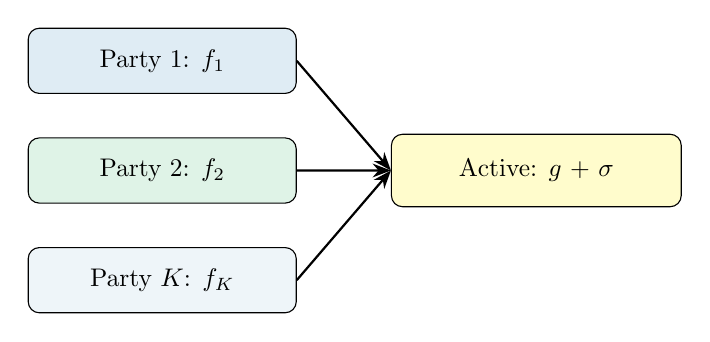
\begin{tikzpicture}[scale=0.92, transform shape]
        \node[draw, rounded corners, fill=vflblue!15, minimum width=3.7cm, minimum height=0.9cm] (p1) {Party 1: $f_1$};
        \node[draw, rounded corners, fill=vflgreen!15, minimum width=3.7cm, minimum height=0.9cm, below=0.6cm of p1] (p2) {Party 2: $f_2$};
        \node[draw, rounded corners, fill=vflblue!8, minimum width=3.7cm, minimum height=0.9cm, below=0.6cm of p2] (pk) {Party $K$: $f_K$};
        \node[draw, rounded corners, fill=yellow!20, minimum width=4.0cm, minimum height=1.0cm, right=1.3cm of p2] (top) {Active: $g$ + $\sigma$};
        \draw[-{Stealth}, thick] (p1.east) -- (top.west);
        \draw[-{Stealth}, thick] (p2.east) -- (top.west);
        \draw[-{Stealth}, thick] (pk.east) -- (top.west);
      \end{tikzpicture}
      \end{center}
      \vspace{0.4em}
      \small Training objective: binary cross-entropy on labels at the active party.
    \end{column}
  \end{columns}
\end{frame}

\begin{frame}{What is ``fine-tuning'' in our project?}
  \begin{block}{Definition (supervisor-proof)}
    \textbf{Fine-tuning (VFU-FT)} means: take the \textbf{already-trained VFL model} and do a few more epochs of training
    \textbf{only on the retain set} \(D_{\text{retain}}\).
  \end{block}
  \vspace{0.6em}
  \begin{exampleblock}{What we fine-tune (in code)}
    We update \textbf{all trainable parameters} (all bottom encoders + the top model) using BCE loss on \(D_{\text{retain}}\)
    (Adam, lr \(\approx 5\times 10^{-4}\), \(\sim 20\) epochs in Part 4).
  \end{exampleblock}
  \vspace{0.4em}
  \begin{alertblock}{What we measure after FT (what should change)}
    \small
    \begin{itemize}
      \item \textbf{Utility}: Accuracy/F1/AUC on test should stay close to before.
      \item \textbf{Forgetting}: MIA AUC on forget-vs-nonmember should move toward \(0.5\) (chance), and forensic detectors should not reliably flag ``unlearned'' behavior.
    \end{itemize}
  \end{alertblock}
  \small Intuition: retain-gradients can overwrite some forget influence, but there is no explicit ``push away'' from forget points.
\end{frame}

\begin{frame}{What is ``KD'' and how does our KD work?}
  \begin{block}{Definition (Knowledge Distillation)}
    \textbf{KD} trains a \textbf{student} model to mimic a \textbf{teacher} model’s outputs while also fitting labels.
    The teacher is the \textbf{original pre-unlearning VFL model} (frozen).
  \end{block}
  \vspace{0.6em}
  \begin{exampleblock}{Our VFU-KD procedure (in code)}
    \begin{itemize}
      \item Build a \textbf{fresh student} (new bottoms + new top).
      \item Compute teacher outputs on \(D_{\text{retain}}\).
      \item Train student on \(D_{\text{retain}}\) using a weighted KD loss (next section).
    \end{itemize}
  \end{exampleblock}
  \vspace{0.4em}
  \begin{alertblock}{What we measure after KD (what should change)}
    \small
    \begin{itemize}
      \item \textbf{Utility}: test metrics remain high (KD tends to preserve the decision boundary).
      \item \textbf{Forgetting}: forget samples become indistinguishable from non-members under MIA; shadow/fuma should have low confidence.
    \end{itemize}
  \end{alertblock}
  \small Why it helps: KD keeps the student close to the teacher’s decision behavior while removing dependence on the forgotten subset (because student never trains on it).
\end{frame}

\begin{frame}{How is unlearning happening in our setup?}
  \begin{block}{Forget setup (Part 4)}
    We sample a forget set \(D_{\text{forget}}\) from the training data (e.g., 5\%) and evaluate
    whether the post-unlearning model is indistinguishable from a \textbf{retain-only} world.
  \end{block}
  \vspace{0.6em}
  \begin{alertblock}{Two unlearning mechanisms we run}
    \begin{itemize}
      \item \textbf{VFU-GA}: gradient ascent on the forget set to \emph{increase} their loss (fast, can hurt utility).
      \item \textbf{VFU-KD}: rebuild student on retain-only with teacher guidance (often best utility).
    \end{itemize}
  \end{alertblock}
  \vspace{0.4em}
  \begin{exampleblock}{We also run VFU-FT (baseline)}
    \small Continue training the same model on \(D_{\text{retain}}\) only (no explicit forgetting objective).
  \end{exampleblock}
\end{frame}

% =============================================================================
\section{(d) Loss function and intuition}
% =============================================================================

\begin{frame}{Base training loss (Phase 0)}
  \begin{block}{Binary cross-entropy (BCE)}
    For label \(y\in\{0,1\}\) and prediction \(\hat{y}\in(0,1)\):
    \[
      \mathcal{L}_{\text{BCE}}(y,\hat{y}) = -y\log(\hat{y})-(1-y)\log(1-\hat{y})
    \]
  \end{block}
  \vspace{0.6em}
  \begin{exampleblock}{Interpretation}
    This is the standard supervised objective that trains all parties jointly through the top model.
  \end{exampleblock}
\end{frame}

\begin{frame}{VFU-GA (Gradient Ascent) loss intuition}
  \begin{block}{What we optimize}
    Normal training: \(\theta \leftarrow \theta - \eta \nabla_\theta \mathcal{L}_{\text{BCE}}\).
    \vspace{0.2em}
    \[
      \textbf{Unlearning (GA):}\quad \theta \leftarrow \theta + \eta \nabla_\theta \mathcal{L}_{\text{BCE}} \ \text{on } D_{\text{forget}}
    \]
  \end{block}
  \vspace{0.6em}
  \begin{alertblock}{Intuition}
    We intentionally make the model \textbf{worse on the forget set only} by \textbf{increasing BCE loss on those samples}.
    In code, we run Adam with lr \(=10^{-3}\) for \(\sim 10\) ascent steps/epochs on \(D_{\text{forget}}\) by backpropagating \(-\mathcal{L}_{\text{BCE}}\).
    This is fast, but can reduce utility and may create detectable ``before→after'' artifacts (what FUMA tries to catch).
  \end{alertblock}
  \vspace{0.3em}
  \begin{exampleblock}{What we measure after GA (what should change)}
    \small
    \begin{itemize}
      \item \textbf{Forget loss} should increase on \(D_{\text{forget}}\) (sanity check that GA is doing what we claim).
      \item \textbf{Membership leakage} should drop: MIA AUC \(\rightarrow 0.5\), gradient-MIA weakens, shadow ``full-data'' probability drops.
    \end{itemize}
  \end{exampleblock}
\end{frame}

\begin{frame}{VFU-KD loss (what exactly we use)}
  \begin{block}{KD objective used in Part 4}
    On retain data, student output \(s\) and teacher output \(t\) are softened by temperature \(T\):
    \[
      p_s = \sigma(s/T),\quad p_t = \sigma(t/T)
    \]
    \[
      \mathcal{L}_{\text{KD}} = \alpha\, T^2\, \mathrm{KL}(p_t \,\|\, p_s) + (1-\alpha)\, \mathcal{L}_{\text{BCE}}(y, \sigma(s))
    \]
  \end{block}
  \vspace{0.5em}
  \begin{exampleblock}{How to explain \(T\) and \(\alpha\)}
    \begin{itemize}
      \item \(T\) smooths probabilities so the student learns teacher ``dark knowledge'' (relative confidence).
      \item \(\alpha\) trades off imitation (KL) vs fitting labels (BCE).
    \end{itemize}
  \end{exampleblock}
\end{frame}

\begin{frame}{Fine-tuning vs KD vs GA (simple mental model)}
  \begin{block}{One-line summaries}
    \begin{itemize}
      \item \textbf{FT}: ``keep training on retain-only'' (overwrite indirectly).
      \item \textbf{KD}: ``rebuild student on retain-only + imitate teacher'' (retain utility, remove forget).
      \item \textbf{GA}: ``push the model away from forget points'' (fast, can be unstable).
    \end{itemize}
  \end{block}
  \vspace{0.6em}
  \begin{alertblock}{Why we still need verification}
    These methods can all look similar on accuracy, but differ on whether they truly remove membership traces.
  \end{alertblock}
\end{frame}

% =============================================================================
\section{(e) Performance report}
% =============================================================================

\begin{frame}{How we report performance (what to look for)}
  \begin{block}{Utility metrics (should stay high)}
    Accuracy / F1 / ROC-AUC on the held-out test set (same split before/after unlearning).
  \end{block}
  \vspace{0.6em}
  \begin{alertblock}{Forgetting / verification signals (should disappear)}
    \begin{itemize}
      \item \textbf{Output MIA (black-box)}: classify member vs non-member using only outputs; \textbf{AUC \(\approx 0.5\)} means indistinguishable.
      \item \textbf{Gradient MIA (stronger access)}: membership signal from gradients/stats; \textbf{AUC \(\approx 0.5\)} is desired.
      \item \textbf{FUMA (forensic)}: detect unlearning by comparing before vs after behavior; \textbf{detection rate \(\rightarrow 0\)} is desired.
      \item \textbf{Shadow model attack}: meta-classifier predicts if model was trained on full vs retain-only; \textbf{Prob(full-data) \(\downarrow\)} is desired.
    \end{itemize}
  \end{alertblock}
  \vspace{0.2em}
  \small In our experiments: \textbf{forget samples} are treated as ``members'' pre-unlearning; we check if they become indistinguishable from held-out/non-member points post-unlearning.
\end{frame}

\begin{frame}{Baseline training behavior (before unlearning)}
  \begin{center}
    \SlideFig{08_training_history_adult.png}{0.90\textwidth}
  \end{center}
  \vspace{0.2em}
  \small This establishes a stable Phase-0 model prior to applying unlearning.
\end{frame}

\begin{frame}{Output MIA (baseline verifier)}
  \begin{center}
    \SlideFig{04_mia_results.png}{0.90\textwidth}
  \end{center}
  \vspace{0.2em}
  \small \textbf{What output is used:} predicted probability/confidence \(\hat{y}\) (or logits) per input; attacker builds features from these outputs
  (e.g., max confidence, entropy, margin, or per-sample loss if labels are known).
  \small \textbf{Measures:} how well an attacker can classify \emph{forget points as training members} vs non-members using only these outputs.
  \small \textbf{Goal:} after unlearning, forget samples should look like non-members (AUC \(\approx 0.5\)).
\end{frame}

\begin{frame}{Gradient MIA (stronger verifier)}
  \begin{center}
    \SlideFig{01_gradient_mia_comparison.png}{0.92\textwidth}
  \end{center}
  \vspace{0.2em}
  \small \textbf{What signal is used:} gradients (or gradient norms/statistics) of the loss w.r.t.\ parameters/embeddings for queried points.
  \small \textbf{Measures:} membership leakage under this stronger access model (AUC \(\approx 0.5\) desired).
  \small Gradient-based signals can detect membership even when output MIA is weak.
\end{frame}

\begin{frame}{FUMA (forensic unlearning detector)}
  \begin{center}
    \SlideFig{03_fuma_results.png}{0.92\textwidth}
  \end{center}
  \vspace{0.2em}
  \small \textbf{What is used:} before-vs-after model responses on points (and derived features from that change).
  \small \textbf{Measures:} whether unlearning leaves a detectable fingerprint (detection rate \(\to 0\) desired).
  \small FUMA asks: ``Can we tell these points were unlearned by comparing before vs after?''
\end{frame}

\begin{frame}{Shadow-model meta attack (model-level fingerprint)}
  \begin{center}
    \SlideFig{05_shadow_attack_results.png}{0.92\textwidth}
  \end{center}
  \vspace{0.2em}
  \small \textbf{What is trained:} a meta-classifier on outputs/features from multiple shadow models trained on full vs retain-only data.
  \small \textbf{Measures:} whether the model globally looks like ``trained on full data'' vs ``retain-only'' (Prob(full-data) \(\downarrow\) desired).
  \small If unlearning is successful, the unlearned model should resemble a retain-only-trained model.
\end{frame}

\begin{frame}{Cross-dataset summary (Part 4)}
  \begin{columns}[T]
    \begin{column}{0.58\textwidth}
      \begin{block}{Why we do this}
        \begin{itemize}
          \item One dataset can be misleading; attacks vary in strength across distributions.
          \item Cross-dataset evaluation supports a clear conclusion: \textbf{verification should be multi-attack and multi-dataset}.
        \end{itemize}
      \end{block}
    \end{column}
    \begin{column}{0.40\textwidth}
      \begin{center}
        \SlideFig{Heatmap_Cross_Dataset.png}{0.98\textwidth}
      \end{center}
    \end{column}
  \end{columns}
\end{frame}

\begin{frame}{Method trade-offs (one visual)}
  \begin{center}
    \SlideFig{Radar_German_Credit.png}{0.92\textwidth}
  \end{center}
  \vspace{0.2em}
  \small Radar summary: utility vs verification behavior across unlearning methods.
\end{frame}

\begin{frame}{Handover}
  \begin{center}
    {\Large \textbf{Next: Feature entanglement and later sections}}\\[0.8em]
    \large (presented by my project partner)
  \end{center}
\end{frame}

\section{(f) Comparison with state-of-the-art}

\begin{frame}{Comparison with related unlearning methods (high level)}
  \small
  \begin{block}{What we compare against (conceptually)}
    \begin{tabular}{@{}p{3.1cm}p{3.7cm}p{5.8cm}@{}}
      \toprule
      \textbf{Line of work} & \textbf{Core idea} & \textbf{Typical limitation (for our goal)} \\
      \midrule
      Retraining / SISA-style & Retrain from scratch or retrain shards & Strong forgetting, but high cost; still needs verification \\
      FedEraser / gradient subtraction (HFL) & Remove historical gradients / calibrated subtraction & Assumes stored gradients + often HFL-oriented \\
      VFL unlearning (VFU-GA / VFU-KD) & GA: maximize loss on forget; KD: student on retain-only & Can look good on accuracy but still leak membership traces \\
      Certified VFL unlearning & Formal guarantees under assumptions & Often stricter assumptions / overhead; still need practical attack evaluation \\
      \bottomrule
    \end{tabular}
  \end{block}
  \vspace{0.5em}
  \begin{exampleblock}{Our contribution in this project}
    We focus on \textbf{verification}: we report a \textbf{standard black-box baseline} (output-based MIA) and add \textbf{stronger/forensic verifiers}
    (Gradient-MIA, FUMA, Shadow) across \textbf{multiple datasets}, to avoid false ``unlearning succeeded'' conclusions.
  \end{exampleblock}
\end{frame}

\section{(g) Challenges / Discussion}

\begin{frame}{Challenges \& discussion (what to say in Q\&A)}
  \begin{block}{Practical challenges}
    \begin{itemize}
      \item \textbf{Utility–privacy trade-off}: strong forgetting (e.g., GA) can harm test performance; KD often preserves utility better.
      \item \textbf{Attack access assumptions}: Gradient-MIA is stronger but assumes gradient/statistics visibility (depends on deployment).
      \item \textbf{Detectable artifacts}: ``before→after'' fingerprints can remain even when output-MIA looks safe (why we include FUMA/Shadow).
      \item \textbf{VFL realism}: we simulate VFL by feature-splitting; real deployments add ID alignment noise, heterogeneity, and system constraints.
    \end{itemize}
  \end{block}
  \vspace{0.4em}
  \begin{alertblock}{Takeaway}
    Always report \textbf{both} utility metrics \textbf{and} multi-attack verification; one number (accuracy) is not sufficient.
  \end{alertblock}
\end{frame}

\begin{frame}{}
  \centering
  {\Large \textbf{Thank you}}\\[0.9em]
  Questions?
\end{frame}

\end{document}

